\section{Introduction}
\label{perception_introduction}

In this chapter a robot is built, which manages to navigate based on its internal sensors only.
This means, it does not use \gls{ac:gps} or externally tracking to compute its own pose.
Furthermore, the here presented approach is entirely data-driven.
Thus, the robot can safely navigate in previously unknown, unstructured indoor or underground environments.


This section divides into two parts.
In the first part, there is a detailed description of a novel denoising filter called \gls{ac:epf}.
In environments with low ambient light conditions, any RGB camera introduces noisy pixels.
The filter removes this noise and replaces it with an averaged value of the local neighborhood.
It is shown that \gls{ac:epf} outperforms standard local denoising methods in quality while still running in real-time.
Global methods, however, show a slightly better performance, but their time performance range at about \unit[0.4]{Hz} and thus are far from real-time (and therefore not feasible in a robotic environment).
As the filter generalizes on any dimension, it can be also used on 1d sensor data, \eg readings from a gyroscope or accelerometer.


This is shown in the second part of this chapter.
Here, two ground based and one flying robot are introduced, which make use of the data filtering.
This enables the robots to use computer vision algorithms to localize themselves and share knowledge about the local environment.
A detailed analysis and comparison to start-of-the art is computed on two simulations: the here developed algorithms perform about twice as good as current state-of-the-art.
Furthermore, real-world office flights are shown.





\subsection{The state-of-the-art of denoising filters}

Real-time computer vision in fast moving robots still remains a challenging task, especially when forced to use limited computing power, as it is usually the case when implemented on embedded systems. 
Different light conditions are just one aspect of this vast field of problems.
Cameras (analog as well as digital cameras) introduce noise in poor light conditions, meaning in environments with low signal-to-noise ratio.
Removing this noise usually leads to better performance of object recognition tasks in 2d and 3d images, more stable computation of features, and improve tracking results.
In~\textcite{reichabramovpapon2013} it was shown  that removal of texture from 2d images significantly improves image segmentation results.
Parts of the results shown here are also published in~\textcite{reichwoergoetterdellen2018}.

An additional application is the automatic post-production of images, which are, generally speaking, more appealing to humans; there is a big community of photographers and we deem removing noise for pure aesthetic value as also important.
One application of the here presented filter is shown in \figref{fig:sensor_introduction_lena}.

Still, the filter generalizes well on arbitrary dimensions.
In a second part it is shown how to apply the same mechanisms to an arbitrary number of dimensions, enabling the filter to run on any physical measurement, for example on 1d sensor data obtained from an accelerometer, gyroscope, or \gls{ac:gps} tracker.

\begin{figure}
    \centering
    \begin{subfigure}[]{0.475\textwidth}
        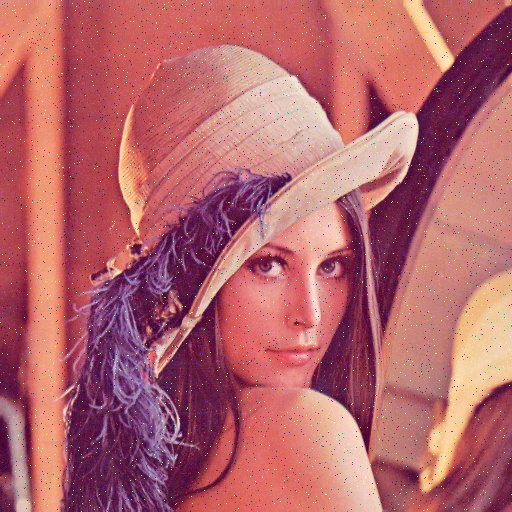
\includegraphics[width=\textwidth]{./figures/sensor/introduction_lena_noisy.jpg}
        \caption{Noisy test image.}
        \label{fig:sensor_introduction_lena_noisy}
    \end{subfigure}\hfill%
    \begin{subfigure}[]{0.475\textwidth}
        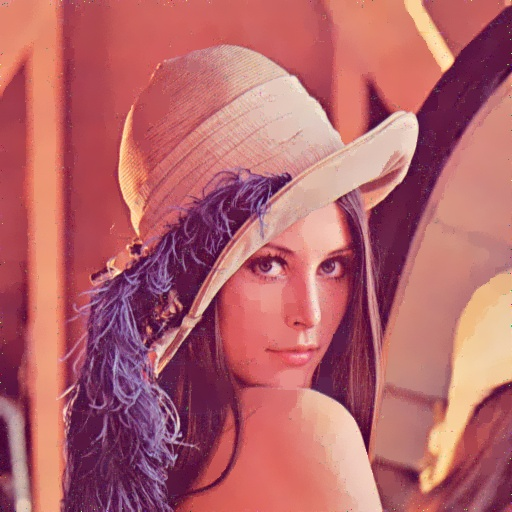
\includegraphics[width=\textwidth]{./figures/sensor/introduction_lena_edgefilter.jpg}
        \caption{Denoised test image.}
        \label{fig:sensor_introduction_lena_denoised}
	\end{subfigure}
  \caption{Even today, denoising remains a challenging task. The here proposed real-time denoising filter is called \gls{ac:epf}.}
  \label{fig:sensor_introduction_lena}
\end{figure}

Removing noise is a two-step process: First a noisy pixel needs to be identified as such, second it needs to be smoothed out. 
Both steps offer a wide range of problems.
In the first step a noisy pixel needs to be defined in a mathematical sense.
This means that a similarity criterion must be found.
However, similarities can exist on different scales, \ie between adjacent pixels or groups of pixels, as it is the case for texture.
In the second step a target value needs to be computed, which replaces the noisy pixel.
This target value should, again, only depend on the local neighborhood.

Removing noise has a long history in science. 
Most notable is the Gaussian Filter. 
It works by convoluting an image with a Gaussian function and thus works as a simple low-pass filter, attenuating high frequency signals~\cite[p. 257f]{gonzalezwoods2002}. 
As edges are also a high-frequency signal, they will be blurred out, too.

Noise in images is usually distinguished using a threshold. 
These thresholds can be either learned using a training set of images, as in support vector machines~\cite{yang2010svm} and \glspl{ac:ann}~\cite{muneyasu1995realization,pandey2016anatomization}, or the threshold may be computed from the surrounding pixel values, as in~\cite{du2011dynamic}. 
\cite{lev1977iterative} identified similar pixels by detecting edges and iteratively replacing the intensity of the pixel by the mean of all pixels in a small environment.

Another approach is presented in~\cite{tomasi1998bilateral}: The so called bilateral filter blurs neighboring pixels depending on their combined color and spatial distance. 
Hence, texture and noise, which has small deviation from the mean can be blurred without affecting boundaries. 
This leads to a trade-off: large blurring factors are needed to smooth out high level of noise, having the consequence that edges are not preserved anymore.

Another wide class of algorithms denoise by averaging. 
This averaging may happen locally as in the Gaussian smoothing model~\cite{lindenbaum1994gabor}, the anisotropic smoothing model~\cite{perona1990scale,alvarez1992image}, based on neighborhood filtering as in the already mentioned bilateral filter~\cite{tomasi1998bilateral}, using local variations as in~\cite{rudin1992nonlinear}, or based on the wavelet thresholding method~\cite{donoho1995noising}.

All these powerful methods have one common drawback: they all smooth small scaled noise and preserve color edges, however are not able to distinguish between a color edge and large scaled noise, \eg outliers. 
Outliers are a common problem in any sensor based application, as in accelerometers or gyroscopes, but also in 2d-RGB cameras, where high ISO settings often pose a big problem. 
More recent methods, which achieve this goal~\cite{dabov2007image,zoran2011learning,mairal2009non}, do not perform in real-time.
The approach presented here has the following features:

\begin{enumerate}
  \item smooths out small scaled noise,
  \item smooths out outliers,
  \item still preserves color edges, and
  \item performs in real-time.
\end{enumerate}





\subsection{The state-of-the-art of Visual Odometry}

The question how an agent using such a filter system behaves in a real-world scenario arises.
A real world agent allows to study behavioral patterns in more details, benchmark, and enhance quality of the algorithms.
The robot's platform should satisfy the following constraints:

\begin{itemize}
  \item the central computing board should be the same for all robots and powerful enough to perform computer vision tasks,
  \item the same code base should be used for all robots; hardware specific specialization should be off-loaded into separate code classes,
  \item sensors should be connectable via modern bus systems such as \wire\ and \ic,
  \item the framework should generalize well and should be easily extensible, and
  \item all robots should be able to communicate with each other via a central \gls{ac:wlan} node or peer-to-peer via Bluetooth.
\end{itemize}

It was decided to use a Raspberry Pi mini computer as computing platform.
Currently, it offers a quad-core \gls{ac:cpu} with \unit[1.4]{GHz}, a memory of \unit[1]{GB} and an onboard Bluetooth and \gls{ac:wlan} chip.
Additionally, an \gls{ac:imu} is attached to all robots, measuring lateral and rotational acceleration.
The robots are shown in \figref{fig:robot_introduction_photo}.
In total, there were two wheeled robots (\figref{fig:robot_introduction_photo_wheelpi}) and one flying robot, \figref{fig:robot_introduction_photo_flypi}, using a quadrotor design, built.

\begin{figure}
  \centering
  \begin{subfigure}[]{0.475\textwidth}
    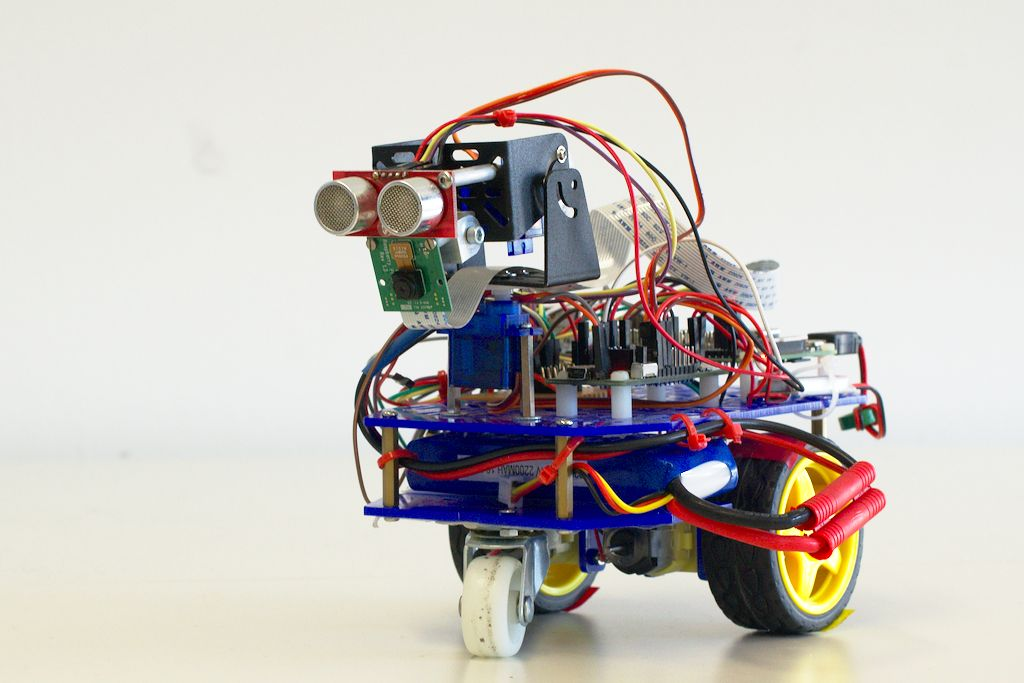
\includegraphics[width=1.0\textwidth]{./figures/robot/photos/wheelpi.jpg}
    \caption{WheelPi robot.}
    \label{fig:robot_introduction_photo_wheelpi}
  \end{subfigure}
  \hfill
  \begin{subfigure}[]{0.475\textwidth}
    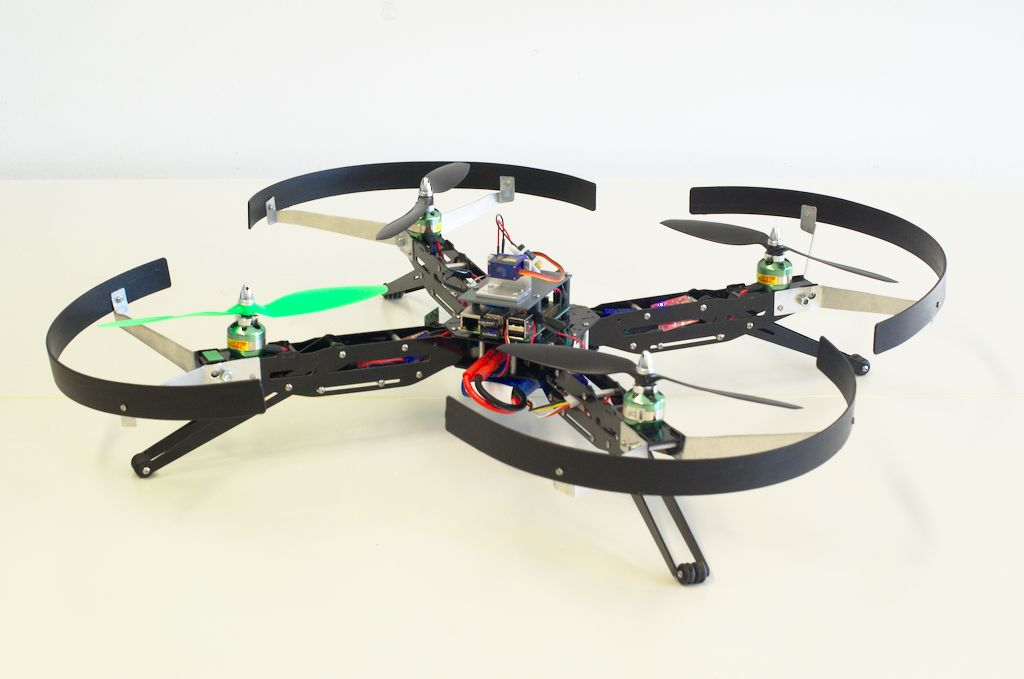
\includegraphics[width=1.0\textwidth]{./figures/robot/photos/quadcopter.jpg}
    \caption{FlyPi robot.}
    \label{fig:robot_introduction_photo_flypi}
  \end{subfigure}
  \caption{The pictures show the robots developed in this work. On the left, there is the WheelPi robot: a three-wheeled ground-based robot. In \figref{fig:robot_introduction_photo_flypi} the FlyPi robot is shown. It is a flying robot utilizing a quadrotor design. Both robots are part of the MovingPi library.}
  \label{fig:robot_introduction_photo}
\end{figure}

Given the constraints from above, the objective of this project is:

\begin{enumerate}
  \item Develop a framework, which can be easily deployed on different hardware designs,
  \item Utilize the framework on multiple agents,
  \item Each agent localizes itself in a previously unknown environment, and
  \item Information about the environment, \ie maps are shared across all agents.
\end{enumerate}

Parts of the here presented work is published in~\textcite{reichseerberscheid2018} and numerous students have contributed to this elaborate project.
They are listed above at the beginning of this thesis.

Humans may easily navigate inside a room.
We have stereo vision, allowing for 3d vision\footnote{At least most of us.}.
We can segment our visual field into subsets, where each subset represents a meaningful entity, \eg. an object.
Because we are able to perform all this intuitively, this is a deceptively tricky business.
One of the pioneers of \gls{ac:ai}, Marvin Minsky, invited to a summer school in 1966 called ``The Summer Vision Project''.
A Memo written by one of his research associates, Seymour Papert, outlines the project goals~\cite[p. 2f]{papert1966summer}:

\begin{enumerate}
  \item ``The primary goal\ldots\ is to\ldots\ divide a\ldots\ picture into regions such as
    \begin{itemize}
      \item likely objects
      \item likely background areas
      \item chaos.''
    \end{itemize}
  \item ``considerable analysis of shape and surface properties'' and ``region description''.
  \item ``The final goal is object identification which will actually name objects by matching them with a vocabulary of known objects.''
\end{enumerate}

Nearly half a century later, \glspl{ac:dnn} have shown promising results towards these goals~\cite{krizhevsky2012imagenet, deng2009imagenet, kim2014convolutional}.
Despite these extensive efforts to solve the ``construction of a significant part of a visual system''~\cite[p. 1]{papert1966summer}, a long road to complete ``computer vision'' remains.
In fact, this is just another form of Moravec's Paradox shown in \secref{ssec:introduction_motivation}; tasks, which are easy for human being are computational expensive for machines.

In this work, the focus lies on fully autonomous robots.
All computations must be performed on embedded hardware, \ie utilizing only limited computational power, and must run online in real-time.
Especially the flying robot, \figref{fig:robot_introduction_photo_flypi}, also named \gls{ac:aav}, must at all times provide safe error propagation and fallback settings.
On embedded hardware, without the support of large multi-core \glspl{ac:cpu} or \glspl{ac:gpu}, robots usually perform with a low frame rate.
One of the most challenging applications is visually guided on-board-com\-pu\-ted indoor flight.
There are no \gls{ac:gps} signals available and the autonomous vehicle has to navigate quickly in confined spaces.
To enable collision detection, onboard sensors have to be utilized.
Truly autonomous robots --- without mandatory connection to a stationary computing system --- and without the need of external sensors for navigation, may be used for example in indoor search-and-rescue missions, disaster relief in dangerous environments (as for example it was the case in Fukushima, Japan, 2011~\cite{chino2011preliminary}), reconnaissance, or underground mining operations.

In recent years, energy efficient, yet powerful hardware and batteries have become available.
Moreover, the physical dimensions of the hardware have been reduced a lot.
This allows on one hand for smaller robots and on the other hand for complex online motor control tasks and sensor evaluation --- as it is required in quadrocopters.
However, active sensor approaches pose the problem of high power consumption and heavy weight.
On today's robots, these problems are solved by using an RGB camera.
RGB cameras are passive sensors with low power consumption.

Previous work on autonomous flight can be categorized into two research areas.
First, many works focus on agile and accurate motion control. Most prominent is the quadrocopter swarm of ETH Zürich, which is able to perform synchronized dancing motions~\cite{schSPRI14}, build simple architectural structures~\cite{augugliaro2014flight}, or even knot strings and build a bridge~\cite{augugliaro2015knot}. 
But these complex tasks heavily rely on external tracking of the robots and are thus restricted to lab use~\cite{brescianini2018trajectory}. 
In another approach, artificial markers in the environment simplify pose estimation~\cite{eberli2011vision}. 
For \gls{ac:gps}-enabled areas, complete commercial solutions exist, \eg~\cite{vasarhelyi2014outdoor,radiansyah2017quadcopter}.

Second, there are approaches, which only use online sensors for self localization.
Still, in many studies the computationally expensive tasks are performed on external hardware via Bluetooth or \gls{ac:wlan} links, \eg~\cite{engel14ras,zhang2016controllable}, which limit the independence of the devices.
In recent years, the miniaturization of computers and advancements in battery design, driven mostly by rapid cell phone development, have made it possible to build smaller autonomous robots and perform computations in real-time on the \gls{ac:aav} itself.
While online computations result in maximum autonomy, even today, real-time computations on 3d data remain a too complex task.
Instead of 3d sensors such as LIDAR, the Asus Xtion Pro, or the Microsoft Kinect sensor, most systems use a monocular camera and perform 3d reconstruction.

For example, the detection of a planar landing zone for a helicopter using a monocular camera was described in~\cite{5584396} in 2010, allowing for autonomous landing of a helicopter.
Following up on this work, seven years later similar results are shown for a moving platform~\cite{falanga2017vision}.
Here, the robot relies only on its internal sensors and lands autonomously on a platform, which holds a marker and moves in a straight line with up to $\unit[4.2]{m/s}$.
\cite{6630807} use a front facing camera to detect objects in the flight path and estimate size.
In recent studies more stable SLAM methods were introduced, \eg~\cite{7219438,engel2014lsd,engel2017direct}, which promise good results for front-facing cameras.
However, these methods are computationally too expensive for embedded hardware.
Also, all approaches with a camera pointing to a specific direction face the problem of a small observation window with significant feature shifts in consecutive camera frames.

Omnidirectional monocular cameras, which provide a 360$\degree$ view of the environment, have been successfully applied to these problems.
Already in 2006 in~\cite{demonceaux2006omnidirectional} full attitude measurements were reported.
\cite{rodriguez2012real} apply this procedure to an unstable flying robot; however, no quantitative results are shown.
In~\cite{lukierski2017room}, a fast moving robot estimates the depth of edges in a corridor using an omnidirectional camera.
In~\cite{forster2014svo} a visual odometry algorithm is introduced, which tracks features and computes frame based pose displacement.
The authors report a frame rate of $\unit[55 \pm 1]{Hz}$, but computations are only performed on certain key frames.

In this work, the focus lies on navigating a flying robot in unknown, GPS-denied, indoor scenarios.
All computations are performed online and in real-time --- there will be no external tracking.
We ask: what is needed to safely (and therefore reliably) detect features on a hardware platform that strongly jerks, jolts, and may even flip?
And --- if those can be found --- how to track them and use them for trajectory planning on limited hardware in real-time?
One goal is to improve navigation by introducing a novel lightweight omnidirectional camera setup for embedded computer systems.
Lastly, the aim is to extract features, track them over multiple frames, compute a 3d point cloud, and perform high level navigation tasks on this internal model of the \gls{ac:aav}'s environment.

In the following section, we shortly introduce our hardware setup, a quadrocopter holding an omnidirectional camera.
Afterwards, the utilized algorithms, called \gls{ac:epf} and \gls{ac:evo}, are introduced.
This is followed by the results section.
First, \gls{ac:epf} is benchmarked on a real-world image data set and, second, experiments on artificial data are shown.
This is followed by three different experiments concerning \gls{ac:evo}: The system is benchmarked using two simulated scenarios and compared to recent methods.
Next, the performance is measured using external cameras to track the robot's position.
Third, a real-world office flight shows the viability of the approach.
The experiments are followed by a detailed discussion and conclusion.
